% TikZ source fragment: activation_learnable.tex
% Included by % TikZ source fragment: activation_learnable.tex
% Included by % TikZ source fragment: activation_learnable.tex
% Included by % TikZ source fragment: activation_learnable.tex
% Included by \input{figures/activation_learnable}.
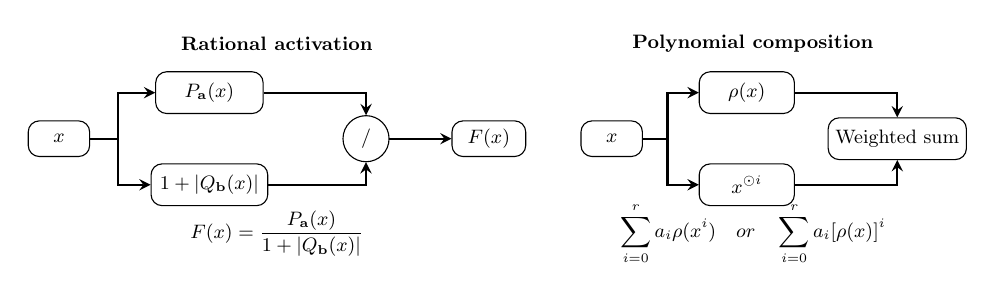
\begin{tikzpicture}[>=stealth, scale=0.78, transform shape, every node/.style={font=\small}]
    % Rational activation panel
    \node[draw, rounded corners, minimum width=1.0cm, minimum height=0.58cm]
        (xr) at (0,0) {$x$};
    \node[draw, rounded corners, minimum width=1.75cm, minimum height=0.68cm]
        (pr) at (2.45,0.75) {\(P_{\mathbf a}(x)\)};
    \node[draw, rounded corners, minimum width=1.9cm, minimum height=0.68cm]
        (qr) at (2.45,-0.75) {\(1+|Q_{\mathbf b}(x)|\)};
    \node[draw, circle, minimum size=0.75cm] (div) at (5.0,0)
        {\(/\)};
    \node[draw, rounded corners, minimum width=1.2cm, minimum height=0.58cm]
        (fr) at (7.0,0) {\(F(x)\)};
    \draw[->, thick] (xr.east) -- ++(0.45,0) |- (pr.west);
    \draw[->, thick] (xr.east) -- ++(0.45,0) |- (qr.west);
    \draw[->, thick] (pr.east) -| (div.north);
    \draw[->, thick] (qr.east) -| (div.south);
    \draw[->, thick] (div) -- (fr);
    \node at (3.55,1.55) {\textbf{Rational activation}};
    \node at (3.55,-1.55)
        {\(\displaystyle F(x)=\frac{P_{\mathbf a}(x)}
        {1+|Q_{\mathbf b}(x)|}\)};

    % Polynomial-composition panel
    \node[draw, rounded corners, minimum width=1.0cm, minimum height=0.58cm]
        (xp) at (9.0,0) {$x$};
    \node[draw, rounded corners, minimum width=1.55cm, minimum height=0.68cm]
        (rho) at (11.2,0.75) {\(\rho(x)\)};
    \node[draw, rounded corners, minimum width=1.55cm, minimum height=0.68cm]
        (pow) at (11.2,-0.75) {\(x^{\odot i}\)};
    \node[draw, rounded corners, minimum width=1.65cm, minimum height=0.68cm]
        (sum) at (13.65,0) {Weighted sum};
    \draw[->, thick] (xp.east) -- ++(0.4,0) |- (rho.west);
    \draw[->, thick] (xp.east) -- ++(0.4,0) |- (pow.west);
    \draw[->, thick] (rho.east) -| (sum.north);
    \draw[->, thick] (pow.east) -| (sum.south);
    \node at (11.3,1.55) {\textbf{Polynomial composition}};
    \node at (11.3,-1.55)
        {\(\displaystyle \sum_{i=0}^{r}a_i\rho(x^i)
        \quad\text{or}\quad
        \sum_{i=0}^{r}a_i[\rho(x)]^i\)};
\end{tikzpicture}
.
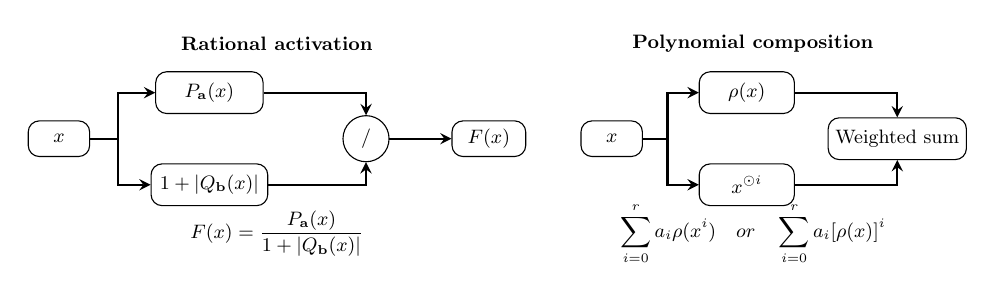
\begin{tikzpicture}[>=stealth, scale=0.78, transform shape, every node/.style={font=\small}]
    % Rational activation panel
    \node[draw, rounded corners, minimum width=1.0cm, minimum height=0.58cm]
        (xr) at (0,0) {$x$};
    \node[draw, rounded corners, minimum width=1.75cm, minimum height=0.68cm]
        (pr) at (2.45,0.75) {\(P_{\mathbf a}(x)\)};
    \node[draw, rounded corners, minimum width=1.9cm, minimum height=0.68cm]
        (qr) at (2.45,-0.75) {\(1+|Q_{\mathbf b}(x)|\)};
    \node[draw, circle, minimum size=0.75cm] (div) at (5.0,0)
        {\(/\)};
    \node[draw, rounded corners, minimum width=1.2cm, minimum height=0.58cm]
        (fr) at (7.0,0) {\(F(x)\)};
    \draw[->, thick] (xr.east) -- ++(0.45,0) |- (pr.west);
    \draw[->, thick] (xr.east) -- ++(0.45,0) |- (qr.west);
    \draw[->, thick] (pr.east) -| (div.north);
    \draw[->, thick] (qr.east) -| (div.south);
    \draw[->, thick] (div) -- (fr);
    \node at (3.55,1.55) {\textbf{Rational activation}};
    \node at (3.55,-1.55)
        {\(\displaystyle F(x)=\frac{P_{\mathbf a}(x)}
        {1+|Q_{\mathbf b}(x)|}\)};

    % Polynomial-composition panel
    \node[draw, rounded corners, minimum width=1.0cm, minimum height=0.58cm]
        (xp) at (9.0,0) {$x$};
    \node[draw, rounded corners, minimum width=1.55cm, minimum height=0.68cm]
        (rho) at (11.2,0.75) {\(\rho(x)\)};
    \node[draw, rounded corners, minimum width=1.55cm, minimum height=0.68cm]
        (pow) at (11.2,-0.75) {\(x^{\odot i}\)};
    \node[draw, rounded corners, minimum width=1.65cm, minimum height=0.68cm]
        (sum) at (13.65,0) {Weighted sum};
    \draw[->, thick] (xp.east) -- ++(0.4,0) |- (rho.west);
    \draw[->, thick] (xp.east) -- ++(0.4,0) |- (pow.west);
    \draw[->, thick] (rho.east) -| (sum.north);
    \draw[->, thick] (pow.east) -| (sum.south);
    \node at (11.3,1.55) {\textbf{Polynomial composition}};
    \node at (11.3,-1.55)
        {\(\displaystyle \sum_{i=0}^{r}a_i\rho(x^i)
        \quad\text{or}\quad
        \sum_{i=0}^{r}a_i[\rho(x)]^i\)};
\end{tikzpicture}
.
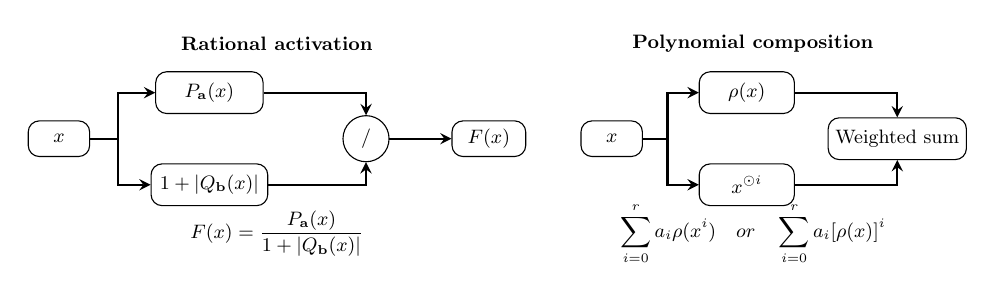
\begin{tikzpicture}[>=stealth, scale=0.78, transform shape, every node/.style={font=\small}]
    % Rational activation panel
    \node[draw, rounded corners, minimum width=1.0cm, minimum height=0.58cm]
        (xr) at (0,0) {$x$};
    \node[draw, rounded corners, minimum width=1.75cm, minimum height=0.68cm]
        (pr) at (2.45,0.75) {\(P_{\mathbf a}(x)\)};
    \node[draw, rounded corners, minimum width=1.9cm, minimum height=0.68cm]
        (qr) at (2.45,-0.75) {\(1+|Q_{\mathbf b}(x)|\)};
    \node[draw, circle, minimum size=0.75cm] (div) at (5.0,0)
        {\(/\)};
    \node[draw, rounded corners, minimum width=1.2cm, minimum height=0.58cm]
        (fr) at (7.0,0) {\(F(x)\)};
    \draw[->, thick] (xr.east) -- ++(0.45,0) |- (pr.west);
    \draw[->, thick] (xr.east) -- ++(0.45,0) |- (qr.west);
    \draw[->, thick] (pr.east) -| (div.north);
    \draw[->, thick] (qr.east) -| (div.south);
    \draw[->, thick] (div) -- (fr);
    \node at (3.55,1.55) {\textbf{Rational activation}};
    \node at (3.55,-1.55)
        {\(\displaystyle F(x)=\frac{P_{\mathbf a}(x)}
        {1+|Q_{\mathbf b}(x)|}\)};

    % Polynomial-composition panel
    \node[draw, rounded corners, minimum width=1.0cm, minimum height=0.58cm]
        (xp) at (9.0,0) {$x$};
    \node[draw, rounded corners, minimum width=1.55cm, minimum height=0.68cm]
        (rho) at (11.2,0.75) {\(\rho(x)\)};
    \node[draw, rounded corners, minimum width=1.55cm, minimum height=0.68cm]
        (pow) at (11.2,-0.75) {\(x^{\odot i}\)};
    \node[draw, rounded corners, minimum width=1.65cm, minimum height=0.68cm]
        (sum) at (13.65,0) {Weighted sum};
    \draw[->, thick] (xp.east) -- ++(0.4,0) |- (rho.west);
    \draw[->, thick] (xp.east) -- ++(0.4,0) |- (pow.west);
    \draw[->, thick] (rho.east) -| (sum.north);
    \draw[->, thick] (pow.east) -| (sum.south);
    \node at (11.3,1.55) {\textbf{Polynomial composition}};
    \node at (11.3,-1.55)
        {\(\displaystyle \sum_{i=0}^{r}a_i\rho(x^i)
        \quad\text{or}\quad
        \sum_{i=0}^{r}a_i[\rho(x)]^i\)};
\end{tikzpicture}
.
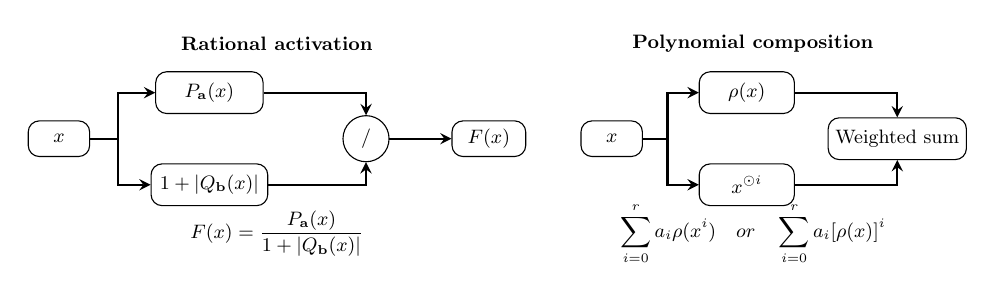
\begin{tikzpicture}[>=stealth, scale=0.78, transform shape, every node/.style={font=\small}]
    % Rational activation panel
    \node[draw, rounded corners, minimum width=1.0cm, minimum height=0.58cm]
        (xr) at (0,0) {$x$};
    \node[draw, rounded corners, minimum width=1.75cm, minimum height=0.68cm]
        (pr) at (2.45,0.75) {\(P_{\mathbf a}(x)\)};
    \node[draw, rounded corners, minimum width=1.9cm, minimum height=0.68cm]
        (qr) at (2.45,-0.75) {\(1+|Q_{\mathbf b}(x)|\)};
    \node[draw, circle, minimum size=0.75cm] (div) at (5.0,0)
        {\(/\)};
    \node[draw, rounded corners, minimum width=1.2cm, minimum height=0.58cm]
        (fr) at (7.0,0) {\(F(x)\)};
    \draw[->, thick] (xr.east) -- ++(0.45,0) |- (pr.west);
    \draw[->, thick] (xr.east) -- ++(0.45,0) |- (qr.west);
    \draw[->, thick] (pr.east) -| (div.north);
    \draw[->, thick] (qr.east) -| (div.south);
    \draw[->, thick] (div) -- (fr);
    \node at (3.55,1.55) {\textbf{Rational activation}};
    \node at (3.55,-1.55)
        {\(\displaystyle F(x)=\frac{P_{\mathbf a}(x)}
        {1+|Q_{\mathbf b}(x)|}\)};

    % Polynomial-composition panel
    \node[draw, rounded corners, minimum width=1.0cm, minimum height=0.58cm]
        (xp) at (9.0,0) {$x$};
    \node[draw, rounded corners, minimum width=1.55cm, minimum height=0.68cm]
        (rho) at (11.2,0.75) {\(\rho(x)\)};
    \node[draw, rounded corners, minimum width=1.55cm, minimum height=0.68cm]
        (pow) at (11.2,-0.75) {\(x^{\odot i}\)};
    \node[draw, rounded corners, minimum width=1.65cm, minimum height=0.68cm]
        (sum) at (13.65,0) {Weighted sum};
    \draw[->, thick] (xp.east) -- ++(0.4,0) |- (rho.west);
    \draw[->, thick] (xp.east) -- ++(0.4,0) |- (pow.west);
    \draw[->, thick] (rho.east) -| (sum.north);
    \draw[->, thick] (pow.east) -| (sum.south);
    \node at (11.3,1.55) {\textbf{Polynomial composition}};
    \node at (11.3,-1.55)
        {\(\displaystyle \sum_{i=0}^{r}a_i\rho(x^i)
        \quad\text{or}\quad
        \sum_{i=0}^{r}a_i[\rho(x)]^i\)};
\end{tikzpicture}
